%\chapter{\normalsize{BACKGROUND OF SATELLITE REMOTE SENSING}}
\chapter{\normalsize{ GOES-R SERIES DATA COLLECTION AND VISUALISATION}}
\section{Acces GOES-R series data files}
\paragraph{}
This section describes few approaches to access, download  and visualise data from GOES-R series satellites.
\subsection{Access data files from NOAA CLASS}
\begin{itemize} 
\item The NOAA \href{https://www.avl.class.noaa.gov/saa/products/welcome}{Comprehensive Large Array-data Stewardship System (CLASS)} repository is the official site for accessing all available GOES-R Series Products.
\item  A similar but easier website to navigate is NCEI's Archive \href{https://www.ncdc.noaa.gov/airs-web/search}{Archive Information Request System (AIRS)}.
\end{itemize}
\subsection{Access data files from Amazon, Microsoft, OCC}
\begin{itemize}
\item \href{https://registry.opendata.aws/noaa-goes/}{Amazon Web Service (AWS)} - ABI L1b and L2+, GLM L2+, and SUVI L1b products are available in AWS S3 Buckets. These open datasets can be accessed by the public from AWS for free. 
\item \href{https://azure.microsoft.com/en-us/services/open-datasets/catalog/goes-16/}{Microsoft Azure}  - Two GOES-16 ABI Full Disk products are stored in a Azure blob container. 
The products currently available are L1b Radiances and L2+ MCMI, which can be accessed from Azure for free.
\item  \href{http://edc.occ-data.org/goes16/}{Open Commons Consortium (OCC)} - Stores a 100 TB rolling archive of GOES-16 data (\~{}8 months), the products stored are ABI L1b and ABI L2+ CMI and MCMI. OCC recommends using the AWS CLI or the python boto library, to access the data. 
\end{itemize}
\subsection{Access data files from Google Cloud}
\begin{itemize}
\item \href{https://console.cloud.google.com/marketplace/product/noaa-public/goes-16?filter=category:science-research&id=5babd633-afa0-4e40-9dba-0587f4aabc47}{Google Cloud} - ABI L1b and L2+, GLM L2+, and SUVI L1b products are available in two different buckets for GOES-16 and GOES-17. 
\item \href{https://developers.google.com/earth-engine}{Google Earth Engine (GEE)} - A cloud-based platform for geospatial analysis. This service runs through 
Google Cloud, and pulls GOES-R datasets from the Google Cloud buckets. 
\end{itemize}
\subsection{Use Python to retrieve data from AWS}
Python is the most powerful programming language using in data science and geospatial data analysis.
The following sample scripts demonstrate how to retrieve GOES-R files from AWS using  Python. 
\begin{lstlisting}[language=Python]
from goespy.Downloader import ABI_Downloader
### to use ABI_Downloader, you need 7 arguments:
import datetime as dt 
### Getting the current date (in UTC coordinate)
utcDateTime = dt.datetime.utcnow() 
## current year
year = utcDateTime.strftime("%Y")
# current month
month = utcDateTime.strftime("%m")
## current day
day = utcDateTime.strftime("%d")
## current hour in UTC 
hour = utcDateTime.strftime("%H")
##Choose a channel from your preference (can be C01-C16)
channel = ["C01"]
## In GOES satellite they have 9 products
## 3 are L1b-Rad(M,C,F)
## 3 are L2-CMIP(M,C,F)
## 3 are L2-MCMIP(M,C,F)
### In your case we will get the CMIPF, F means FullDisk (all the projection by the satellite)
product = 'L1b-L2-CMIPF'
## The Bucket is the variable contains the name of dataset server from goes on AWS
Bucket = 'noaa-goes16' ## in the future on AWS they will have goes17.
## Now we will call the function ABI_Downloader:
Abi = ABI_Downloader('noaa-goes16',year,month,day,hour,product,channel)
\end{lstlisting}
After all the dataset is downloaded, they are in your home directory with that structure:
\begin{figure}[H]
\begin{center}
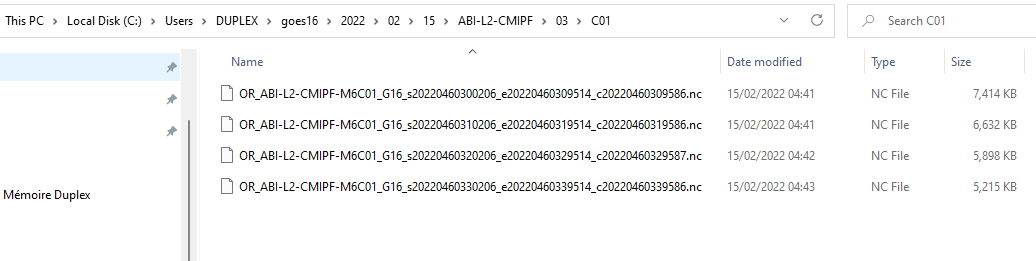
\includegraphics[scale=0.6]{file1.png} %\cite{umhe}
\end{center}
\caption{L1b-L2-CMIPF product downloaded}
\label{L1b-L2-CMIPF product downloaded}%\cite{ABIA}
\end{figure}
\section{GOES-R Series metadata discovery}
\subsection{ GOES-R Series data format}
GOES-R Series product files use the netCDF-4 format.
Network Common Data Form (NetCDF) is a set of software libraries and machine-independent data formats that support the creation, access, and sharing of array-oriented scientific data. It is also a community standard for sharing scientific data.
\subsection{Read GOES-R Series data metadata}
Metadata provides information about the distinct items, such as: means of creation, purpose of 
the data, time and date of creation, creator or author of data, placement on a network (electronic 
form) where the data was created, what standards used etc.
The main purpose of metadata is to facilitate in the discovery of relevant information, more often 
classified as resource discovery. Metadata also helps organize electronic resources, provide 
digital identification, and helps support archiving and preservation of the resource.
Before any manipulation of data, it is vitaly important to read metadata.
Now let us see how to read the metadata of this satellite data file in command line using gdal tools.
\begin{lstlisting}[language=Bash]
## change directory to where you have downloaded the GLDAS data using the below
cd /mnt/d/MI_IS_DATA_ANALYSIS
## extatract metadata of the 'OR_ABI-L1b-RadM1-M3C02_G16_s20171931811268_e20171931811326_c20171931811356.nc' 
gdalinfo OR_ABI-L1b-RadM1-M3C02_G16_s20171931811268_e20171931811326_c20171931811356.nc
## press enter
\end{lstlisting}
\begin{figure}[H]
\begin{center}
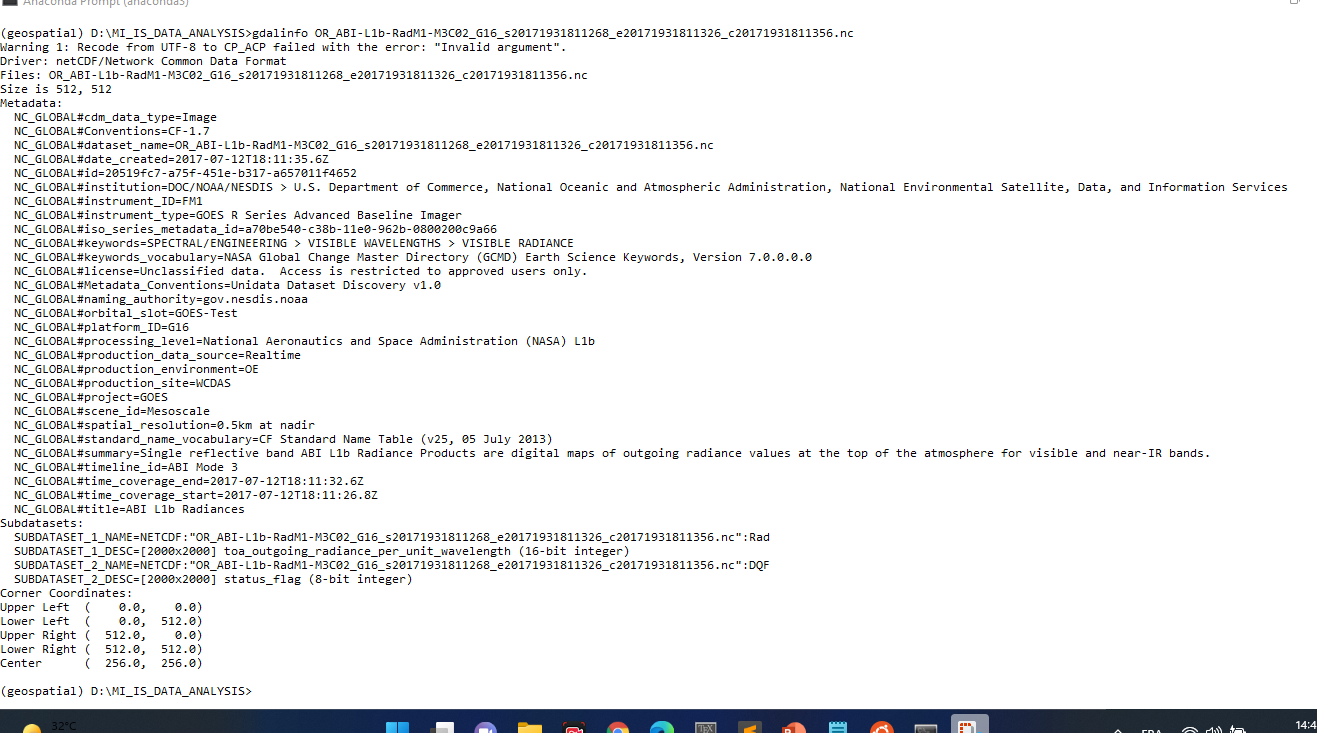
\includegraphics[scale=0.5]{gdal1.png} %\cite{umhe}
\end{center}
\caption{GOES-R Series metadata discovery}
\label{GOES-R Series metadata discovery}%\cite{ABIA}
\end{figure}

\section{Visualise a single band ABI Channel image}
ABI imager has 16 channels, the code below show how to plot a single band ABI channel image.
\begin{lstlisting}[language=Python]
def open_dataset(date, channel, idx, region):
    """
    Open and return a netCDF Dataset object for a given date, channel, and image index
    of GOES-16 data from THREDDS test server.
    """
    cat = TDSCatalog('https://thredds.ucar.edu/thredds/catalog/satellite/goes/east/products/'
                     f'CloudAndMoistureImagery/{region}/Channel{channel:02d}/{date:%Y%m%d}/catalog.xml')
    ds = cat.datasets[idx]
    ds = ds.remote_access(use_xarray=True)   
    return ds
def plot_GOES16_channel(date, idx, channel, region):
    """
    Get and plot a GOES 16 data band from the ABI.
    """
    ds = open_dataset(date, channel, idx, region)
    dat = ds.metpy.parse_cf('Sectorized_CMI')
    proj = dat.metpy.cartopy_crs
    x = dat['x']
    y = dat['y']
    fig = plt.figure(figsize=(10, 10))
    ax = fig.add_subplot(1, 1, 1, projection=proj)
    ax.add_feature(cfeature.COASTLINE, linewidth=2)
    ax.add_feature(cfeature.STATES, linestyle=':', edgecolor='black')
    ax.add_feature(cfeature.BORDERS, linewidth=2, edgecolor='black')
    for im in ax.images:
        im.remove()
    im = ax.imshow(dat, extent=(x.min(), x.max(), y.min(), y.max()), origin='upper')
    timestamp = datetime.strptime(ds.start_date_time, '%Y%j%H%M%S')
    add_timestamp(ax, time=timestamp, high_contrast=True, 
                  pretext=f'GOES 16 Ch.{channel} - ',
                  time_format='%d %B %Y %H%MZ', y=0.01,
                  fontsize=18)
    display(fig)
    plt.savefig("goes_fulldisk_C1.png")
    plt.close()
channel_list = {u'1 - Blue Band 0.47 \u03BCm': 1,
                u'2 - Red Band 0.64 \u03BCm': 2,
                u'3 - Veggie Band 0.86 \u03BCm': 3,
                u'4 - Cirrus Band 1.37 \u03BCm': 4,
                u'5 - Snow/Ice Band 1.6 \u03BCm': 5,
                u'6 - Cloud Particle Size Band 2.2 \u03BCm': 6,
                u'7 - Shortwave Window Band 3.9 \u03BCm': 7,
                u'8 - Upper-Level Tropo. WV Band 6.2 \u03BCm': 8,
                u'9 - Mid-Level Tropo. WV Band 6.9 \u03BCm': 9,
                u'10 - Low-Level WV Band 7.3 \u03BCm': 10,
                u'11 - Cloud-Top Phase Band 8.4 \u03BCm': 11,
                u'12 - Ozone Band 9.6 \u03BCm': 12,
                u'13 - Clean IR Longwave Band 10.3 \u03BCm': 13,
                u'14 - IR Longwave Band 11.2 \u03BCm': 14,
                u'15 - Dirty Longwave Band 12.3 \u03BCm': 15,
                u'16 - CO2 Longwave IR 13.3 \u03BCm': 16}
region = Select(
    options=['Mesoscale-1', 'Mesoscale-2', 'CONUS', 'PuertoRico', 'FullDisk'],
    description='Region:',)

channel = Dropdown(options=channel_list,value=16,description='Channel:',)

interact(plot_GOES16_channel, date=fixed(date), idx=fixed(-2), 
         channel=channel, region=region)

\end{lstlisting}

\begin{figure}[h!]
%\begin{figure}[H]
%\begin{figure}[t]
%\begin{figure}[b]
%\begin{figure}[b]
  \centering
  \begin{subfigure}[a]{0.8\linewidth}
    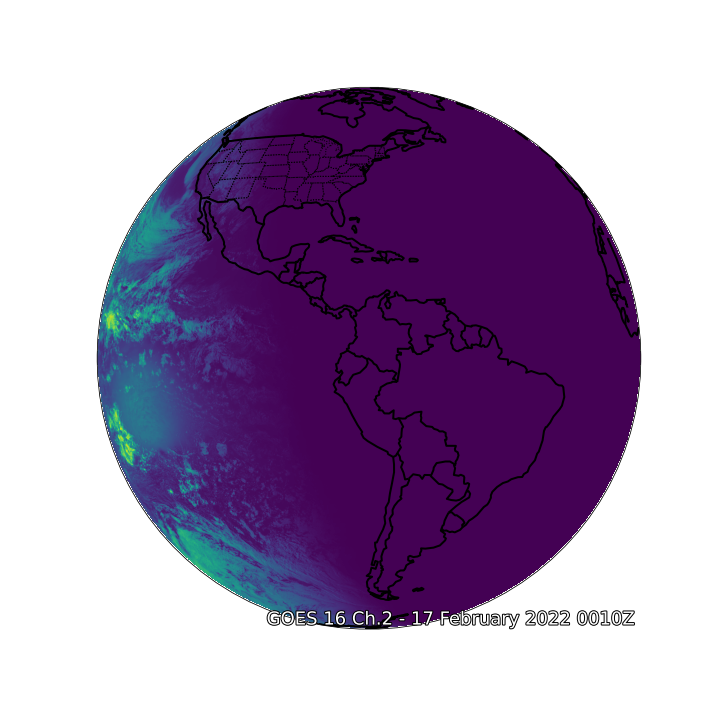
\includegraphics[width=\linewidth]{goes_fulldisk_C01.png}
     \caption{ABI channel 1 image full disk}
  \end{subfigure}
   %\centering
  \begin{subfigure}[b]{0.4\linewidth}
    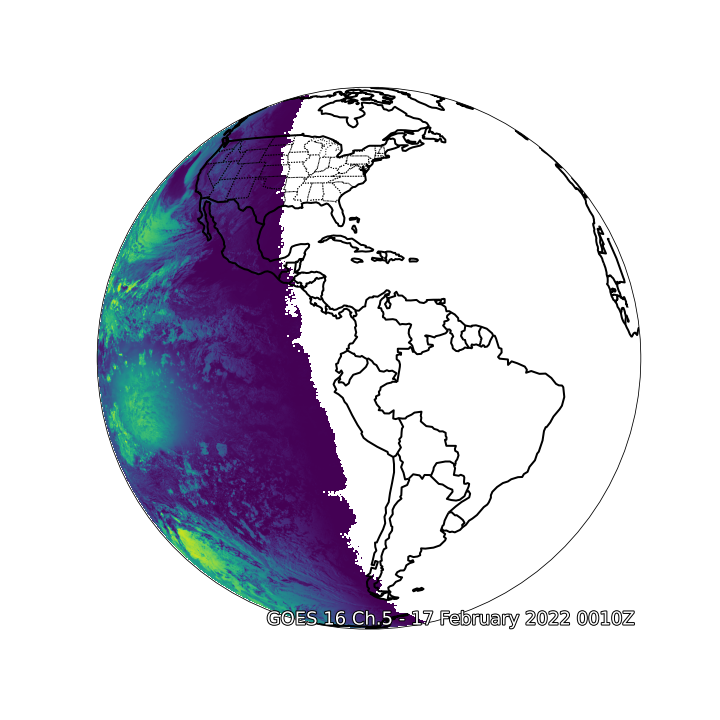
\includegraphics[width=\linewidth]{goes_fulldisk_C05.png}
    \caption{ABI channel 5 image full disk}
  \end{subfigure}
   %\centering
   %\centering
  \begin{subfigure}[b]{0.4\linewidth}
    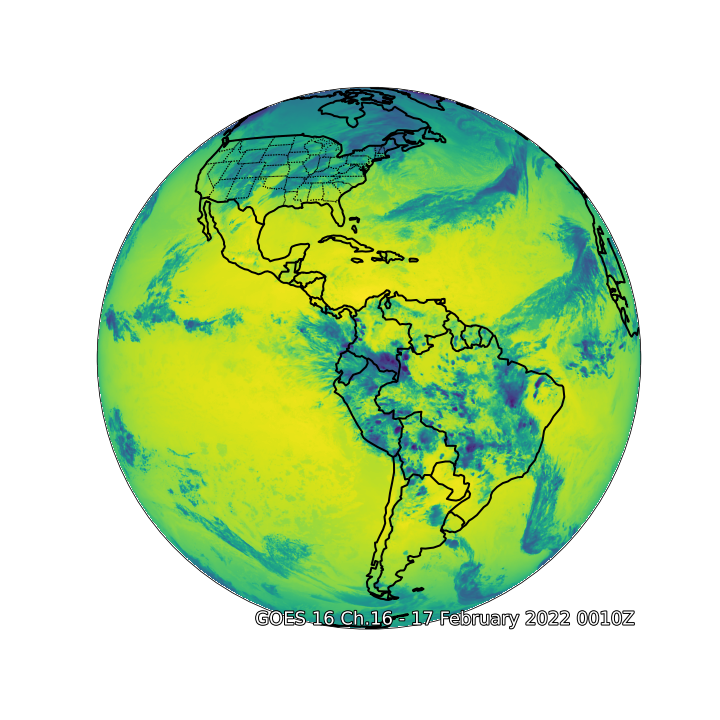
\includegraphics[width=\linewidth]{goes_fulldisk_C16.png}
    \caption{ABI channel 16 image full disk}
  \end{subfigure}
  \caption{ABI images full disk}
  \label{ABI images full disk}
\end{figure}
